\documentclass[compress]{beamer}
%\documentclass[compress,handout]{beamer}

%%%%% PREAMBLE %%%%%

% we want to draw diagrams (turns out not like this though)
\usepackage{tikz}

% figures in a presentation look better without "Figure"
\usepackage{caption}
\captionsetup[figure]{labelformat=empty}

%% % for Idris syntax highlighting
%% \usepackage[styles]{idrislang}

\usepackage{minted}
\setminted{
  fontsize=\small,
  breaklines=true
}

% slide url at the end
\usepackage{hyperref}
\hypersetup{
  colorlinks=true,
  urlcolor=purple
}

% N.B. For some reason, things don't build without this...
\usepackage{todonotes}
\setuptodonotes{inline} % for things to work nicely with beamer

\usetheme{metropolis}

\title{Type-Level Property Based Testing}

\author{{\bfseries Thomas Ekstr{\" o}m Hansen} \& Edwin Brady}
\date{TyDe '24 {\textemdash} 9\textsuperscript{th} September 2024}

\definecolor{highl}{HTML}{dafc5f}
\definecolor{staBlue}{HTML}{00539b}
\definecolor{staMidGreen}{HTML}{00853f}
\definecolor{staDarkGreen}{HTML}{005953}
\setbeamercolor{frametitle}{bg=staDarkGreen}


%%%%% DOCUMENT %%%%%

% /!\     N.B.: `fragile` required for listing to work     /!\

\begin{document}

\maketitle


%% MARK: Motivation
\begin{frame}
  \frametitle{Motivation}

  \large

  \begin{itemize}
    \item<1-> Many systems exhibit Finite-State-Machine-like behaviour
    \item<2-> These can be modelled using dependent types
    \begin{itemize}
      \item<3-> Dependent types are difficult to get right
    \end{itemize}
    \item<4-> How do we increase confidence in our dependent types?
  \end{itemize}

\end{frame}


%% MARK: Disclaimer
\begin{frame}
  \frametitle{Disclaimer: ``increase confidence''}

  \begin{center}
    {\Large
    This is not a proof technique
    }

    {\large
    But hopefully, it helps us catch errors faster and provides guarantees that
    our model behaves as intended
    }
  \end{center}

\end{frame}


%% MARK: Stateful systems
\begin{frame}
  \frametitle{Stateful Computer Systems}

  \large

  \begin{itemize}
    \item<1-> Stateful systems are ubiquitous
    \item<2-> Embedded controllers for automatic doors, ATMs, network protocols,
              etc...
    \item<3-> These are all stateful
    \item<4-> And we would very much like them to be correct
  \end{itemize}

\end{frame}


%% MARK: Spectrum
\begin{frame}[fragile]
  \frametitle{Spectrum of Verification}

  \hspace*{-5mm}  % to fit the bounding box of the tikz diagram
  % ~~probably~~ DEFINITELY cursed
  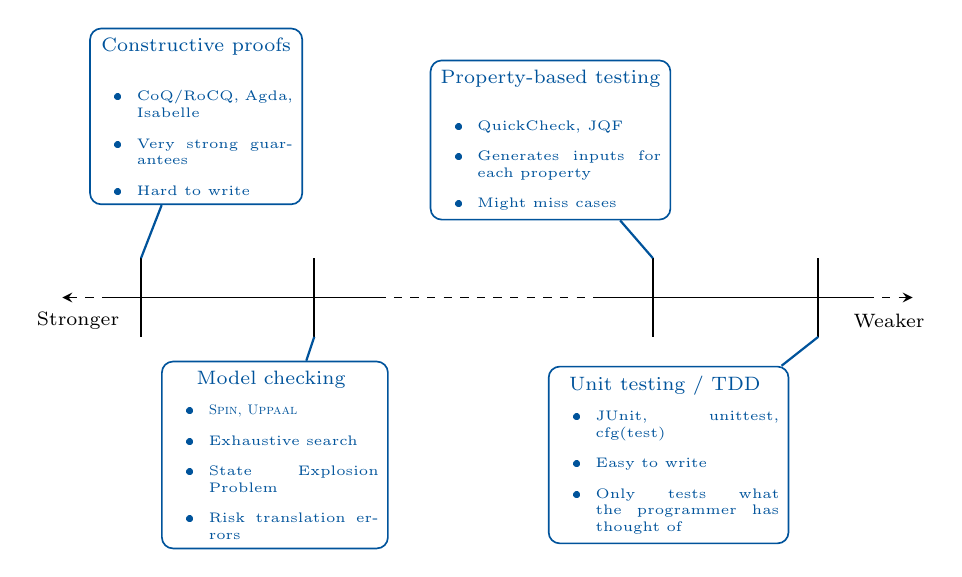
\begin{tikzpicture}[> = stealth, semithick]
    % scale %

    % left half
    \draw [dashed, <-] (-0.2, 0) -- (0.4, 0) ;
    \draw (0.4, 0) -- (3.8, 0) ;

    % middle dashed
    \draw [dashed] (3.8, 0) -- (6.6, 0) ;

    % right half
    \draw (6.6, 0) -- (10, 0) ;
    \draw [dashed, ->] (10, 0) -- (10.6, 0) ;


    % ticks / vertical lines %

    % leftmost tick (constructive proofs)
    \draw<2-> (0.8, -0.5) -- (0.8, 0.5) ;
    
    % tick for model checking
    \draw<3-> (3, -0.5) -- (3, 0.5) ;

    % tick for Quickcheck
    \draw<4-> (7.3, -0.5) -- (7.3, 0.5) ;

    % rightmost tick (unit tests)
    \draw<5-> (9.4, -0.5) -- (9.4, 0.5) ;


    % scale labels %

    \node at (0, -0.3) {\scriptsize Stronger} ;
    \node at (10.3, -0.3) {\scriptsize Weaker} ;


    % text boxes with arrows %

    % constructive proofs
    \node<2->
          [draw, rounded corners,
          text width=7em,
          align=flush center,
          color=staBlue]% 
          at (1.5, 2.3)
          (tbox-prf)
          \bgroup
          \scriptsize
          Constructive proofs
          \vspace*{-2pt}
          \tiny
          % LaTeX looks beautiful and nice
          % Also LaTeX:
          \setlength{\leftmargini}{2em}
          \begin{itemize}%[leftmargin=*]
            \item CoQ/RoCQ, Agda, Isabelle \vspace*{-3pt}
            \item Very strong guarantees \vspace*{-3pt}
            \item Hard to write
          \end{itemize}
          \egroup
          ;
    \draw<2-> [thick, color=staBlue] (tbox-prf) -- (0.8, 0.5) ;

    % model checking
    \node<3->
          [draw, rounded corners,
          text width=7.5em,
          align=flush center,
          color=staBlue]% 
          at (2.5, -2)
          (tbox-mc)
          \bgroup
          \scriptsize
          Model checking
          \vspace*{-3pt}
          \tiny
          \setlength{\leftmargini}{2em}
          \begin{itemize}%[leftmargin=*]
            \item \textsc{Spin, Uppaal}  \vspace*{-3pt}
            \item Exhaustive search  \vspace*{-3pt}
            \item State Explosion Problem  \vspace*{-3pt}
            \item Risk translation errors
          \end{itemize}
          \egroup
          ;
    \draw<3-> [thick, color=staBlue] (tbox-mc) -- (3, -0.5) ;

    % property-based testing
    \node<4->
          [draw, rounded corners,
          text width=8em,
          align=flush center,
          color=staBlue]% 
          at (6, 2)
          (tbox-qc)
          \bgroup
          \scriptsize
          Property-based testing
          \vspace*{-3pt}
          \tiny
          \setlength{\leftmargini}{2em}
          \begin{itemize}%[leftmargin=*]
            \item QuickCheck, JQF \vspace*{-3pt}
            \item Generates inputs for each property \vspace*{-3pt}
            \item Might miss cases
          \end{itemize}
          \egroup
          ;
    \draw<4-> [thick, color=staBlue] (tbox-qc) -- (7.3, 0.5) ;

    % tdd
    \node<5->
          [draw, rounded corners,
          text width=8em,
          align=flush center,
          color=staBlue]% 
          at (7.5, -2)
          (tbox-tdd)
          \bgroup
          \scriptsize
          Unit testing / TDD
          \vspace*{-3pt}
          \tiny
          \setlength{\leftmargini}{2em}
          \begin{itemize}%[leftmargin=*]
            \item JUnit, unittest, cfg(test) \vspace*{-3pt}
            \item Easy to write \vspace*{-3pt}
            \item Only tests what the programmer has thought of
          \end{itemize}
          \egroup
          ;
    \draw<5-> [thick, color=staBlue] (tbox-tdd) -- (9.4, -0.5) ;

  \end{tikzpicture}

\end{frame}


%% MARK: TyDe
\begin{frame}[fragile]
  \frametitle{What about Type-Driven Development?}

  \large

  \begin{columns}
  \begin{column}{0.6\framewidth}
    \begin{itemize}
      \item<1-> Dependently typed languages like Agda and Idris
      \item<2-> Can construct advanced types and embedded DSLs
      \item<3-> Have the types and type checker guide the implementation and
                verify its behaviour (correct-by-construction)
    \end{itemize}
  \end{column}
  \begin{column}{0.4\framewidth}
    \begin{onlyenv}<4->
    \begin{minted}[gobble=6,fontsize=\normalsize,breaklines=false]{Haskell}
      head :: [a] -> a
      -- crashes on
      -- `head []`
    \end{minted}
    \end{onlyenv}

    \vspace*{3mm}

    \begin{onlyenv}<5->
    \begin{minted}[gobble=6,fontsize=\normalsize,breaklines=false]{Idris}
      head :  Vect (S k) a
           -> a
      -- always safe because
      -- the length must be
      -- at least 1
    \end{minted}
    \end{onlyenv}
  \end{column}
  \end{columns}

  \vspace*{2mm}
  \begin{onlyenv}<6->
  \begin{center}
    \large
    Fits somewhere in the middle
  \end{center}
  \vspace*{-12mm}
  \end{onlyenv}

\end{frame}


%% MARK: ATM Diagram
\begin{frame}
  \frametitle{The ATM state machine}

  \begin{figure}
    \centering
    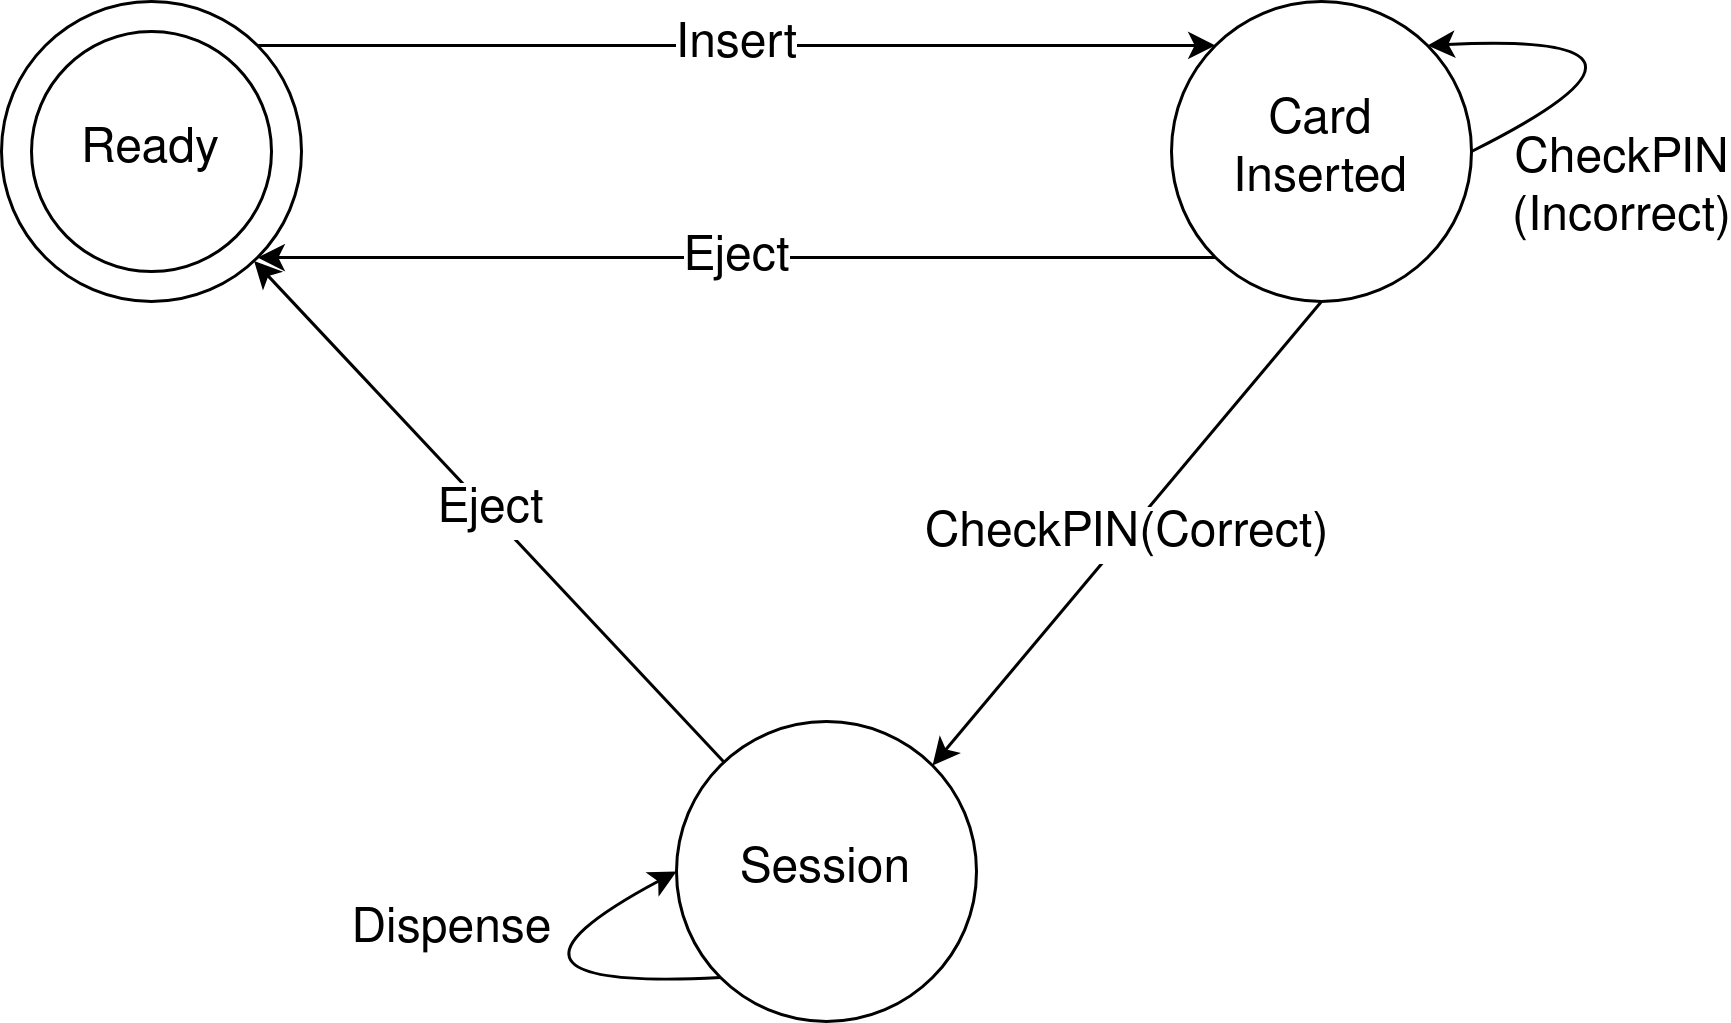
\includegraphics[alt={A state diagram of an ATM, with circles for each state: Ready, CardInserted, and Session; labelled arrows between the states; with the labels containing the transition names: Insert, Dispense, CheckPIN(Correct), CheckPIN(Incorrect), and Eject.},width=0.8\framewidth]{ATM.png}
    %% \Description{A state diagram of an ATM, with circles for each state: Ready,
    %%              CardInserted, and Session; labelled arrows between the states;
    %%              with the labels containing the transition names: Insert,
    %%              Dispense, CheckPIN(Correct), CheckPIN(Incorrect), and Eject.}
  \end{figure}
  \vspace*{-1cm}

\end{frame}


%% Edwin: cut?
%% MARK: ATM States
\begin{frame}[fragile]
  \frametitle{Datatype for the ATM states}

  \begin{columns}
  \begin{column}{0.3\framewidth}
    \begin{minted}[gobble=6,fontsize=\normalsize]{Idris}
      data ATMState
        = Ready
        | CardInserted
        | Session
    \end{minted}
  \end{column}

  \begin{column}{0.65\framewidth}
    \begin{figure}
    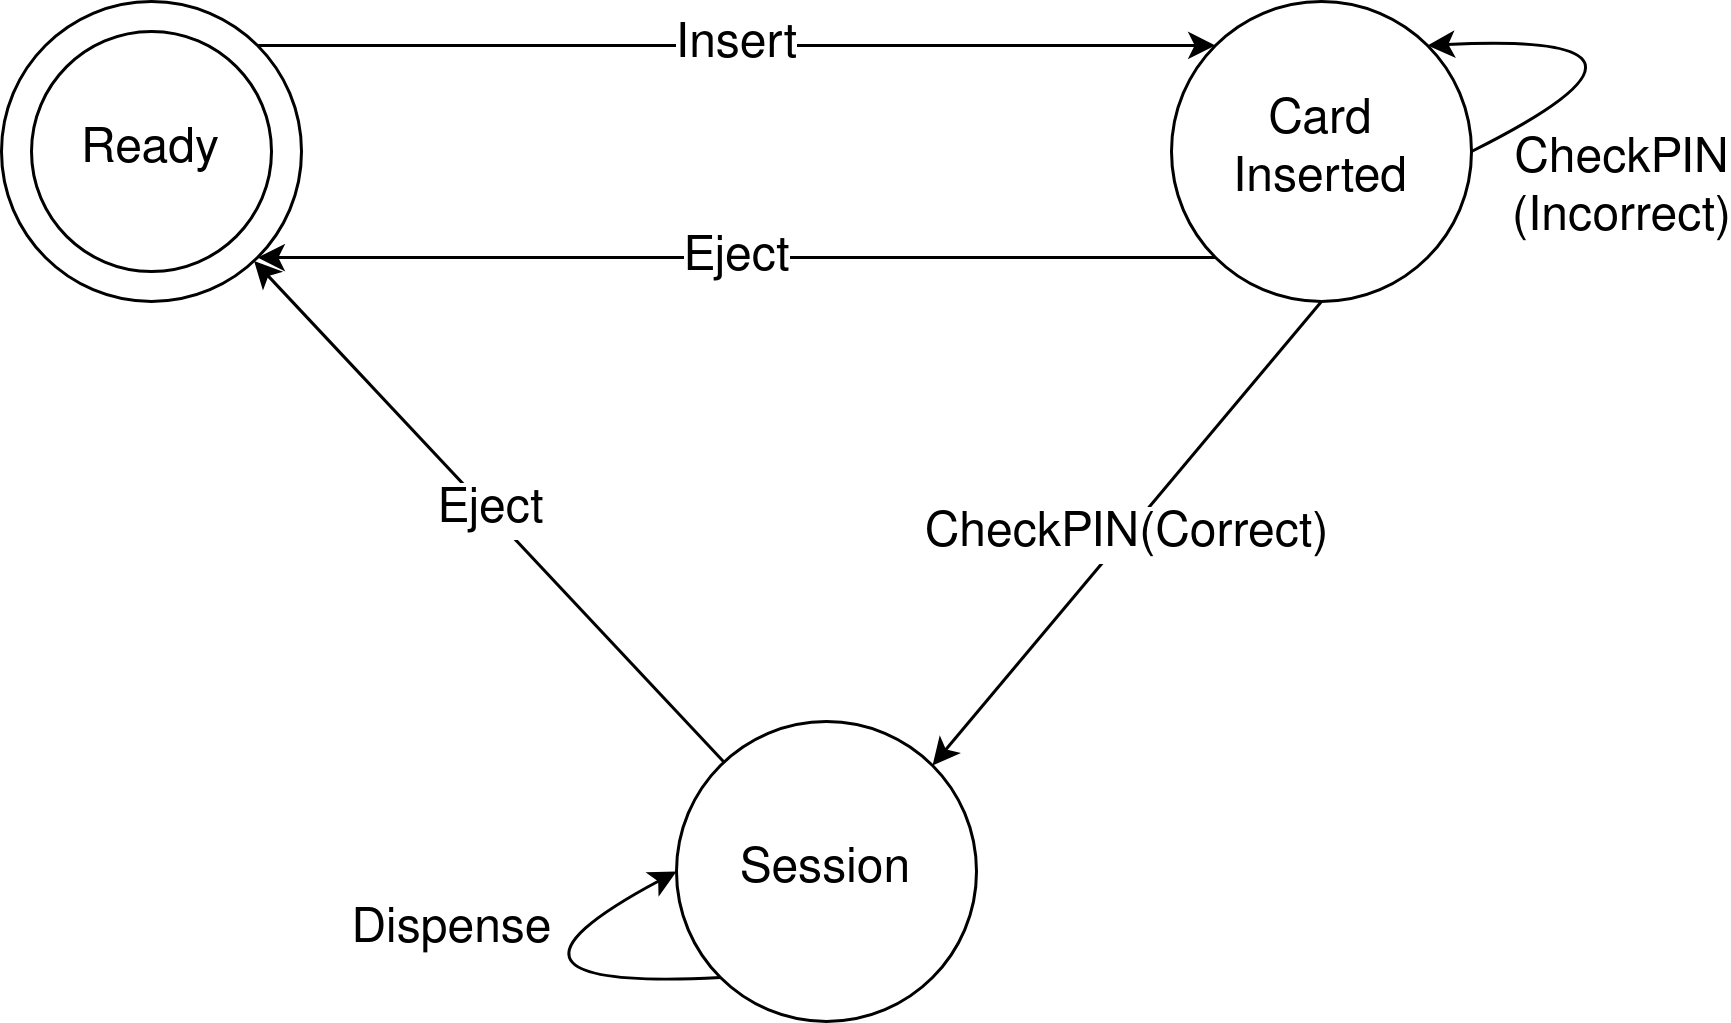
\includegraphics[alt={The state diagram from slide 7.},width=\textwidth]{ATM.png}
    %% \Description{The ATM diagram from slide 7}
    \end{figure}
  \end{column}
  \end{columns}

\end{frame}


%% Edwin: cut?
%% MARK: ATM Results
\begin{frame}[fragile]
  \frametitle{Datatype for ATM operation results}

  \begin{columns}
  \begin{column}{0.3\framewidth}
    \begin{minted}[gobble=6,fontsize=\normalsize]{Idris}
      data PINok 
        = Correct
        | Incorrect
    \end{minted}
  \end{column}

  \begin{column}{0.65\framewidth}
    \begin{figure}
    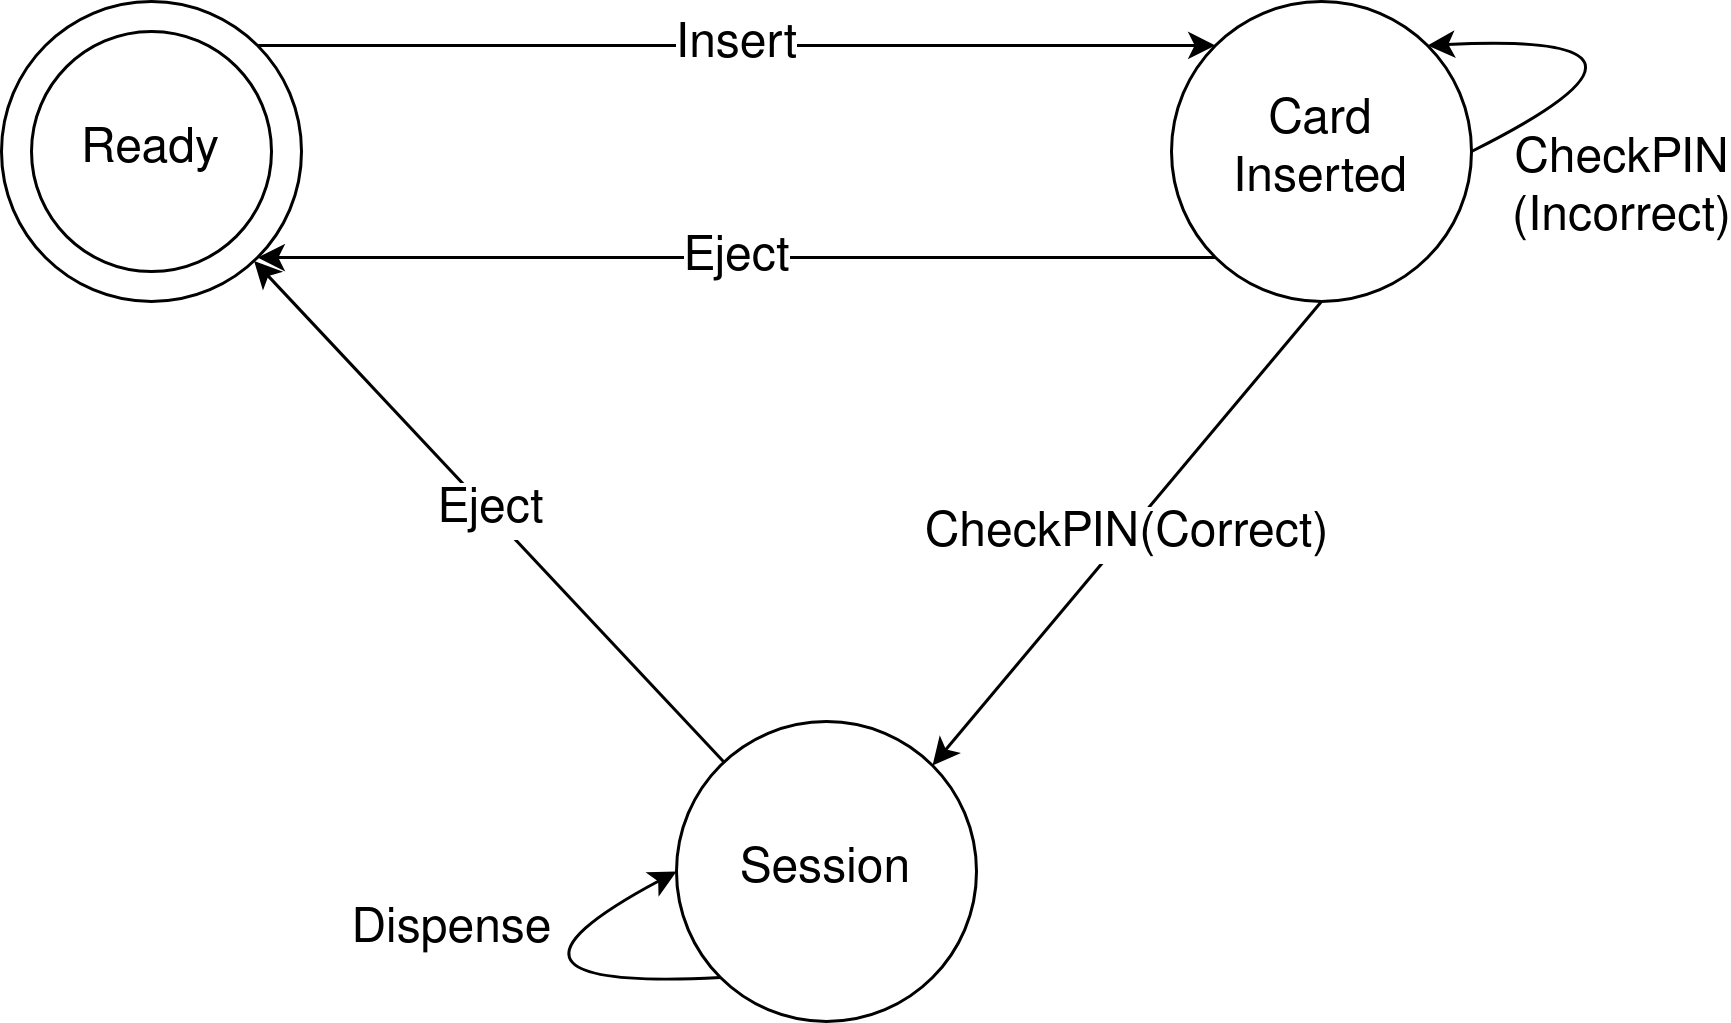
\includegraphics[alt={The state diagram from slide 7.},width=\textwidth]{ATM.png}
    %% \Description{The state diagram from slide 7.}
    \end{figure}
  \end{column}
  \end{columns}

  \vspace*{1cm}

  \pause

  \large

  Everything which does not have a result returns Unit {\textemdash}
  \mintinline{Idris}|()|

\end{frame}


%% MARK: ChkPINfn
\begin{frame}[fragile]
  \frametitle{State Transition Function}

  \begin{columns}
  \begin{column}{0.5\framewidth}
    \begin{minted}[gobble=6]{Idris}
      ChkPINfn : PINok -> ATMState
      ChkPINfn Correct = Session
      ChkPINfn Incorrect = CardInserted
    \end{minted}
  \end{column}
  \hspace*{-7mm}
  \begin{column}{0.55\framewidth}
    \begin{figure}
    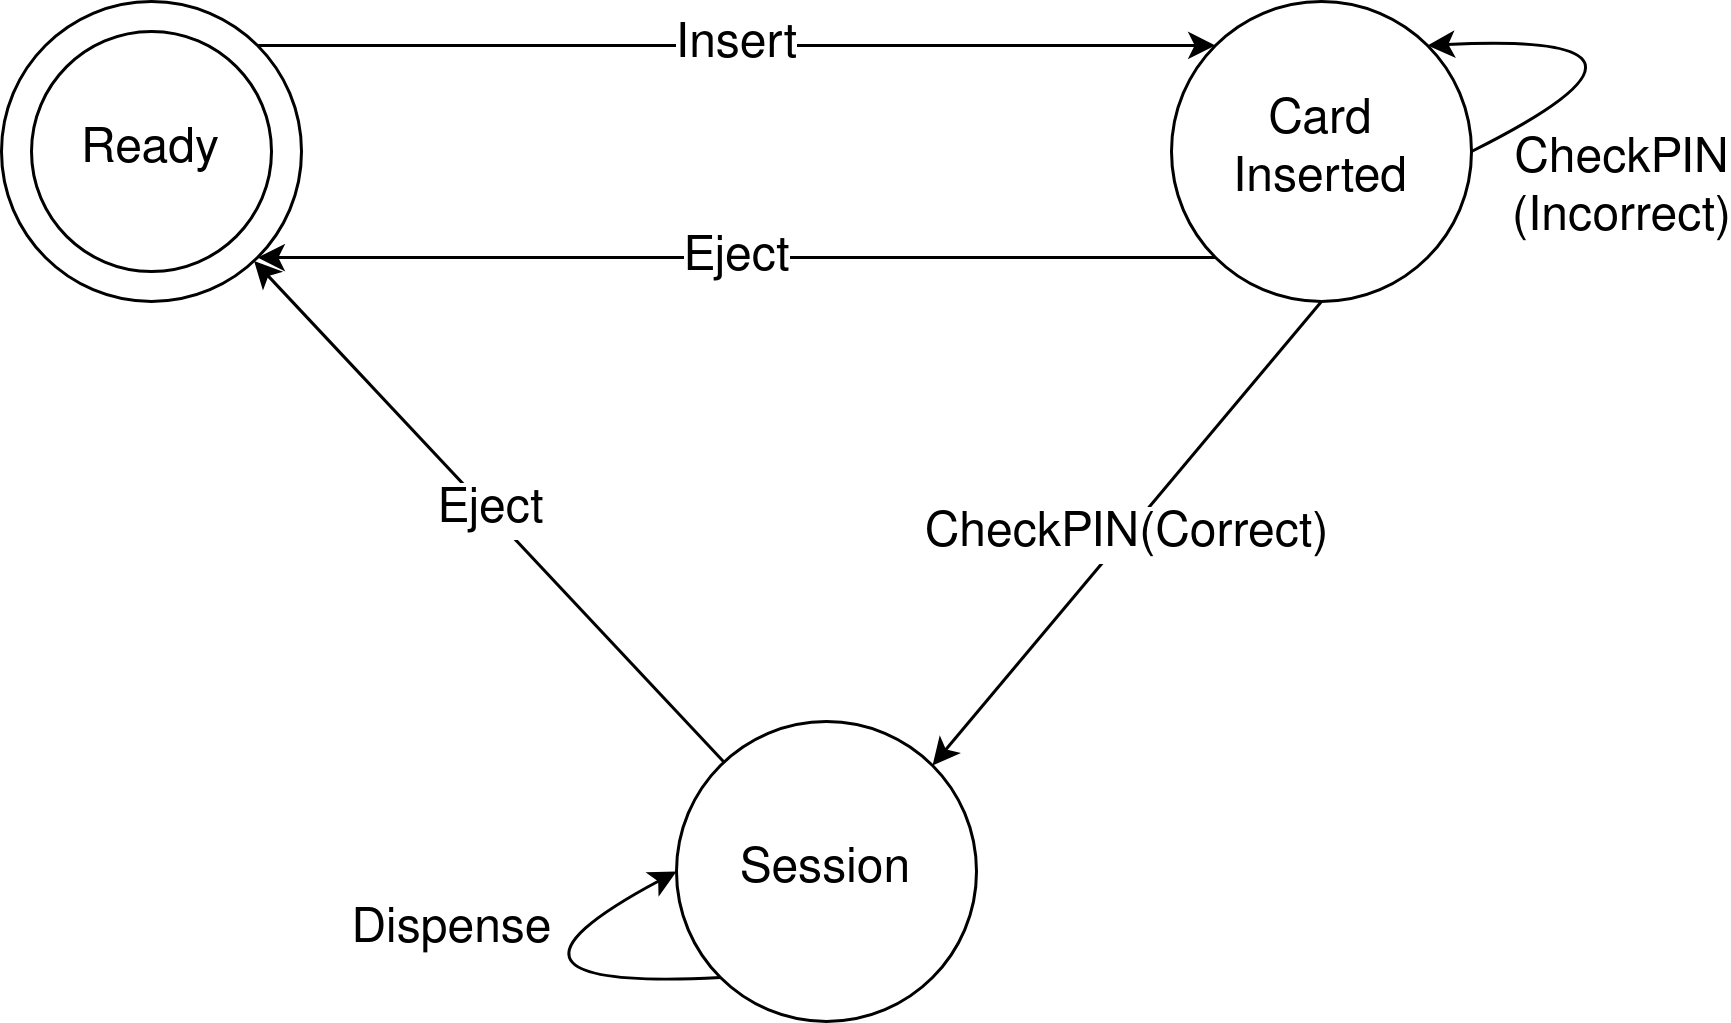
\includegraphics[alt={The state diagram from slide 7.},width=\textwidth]{ATM.png}
    %% \Description{The state diagram from slide 7.}
    \end{figure}
  \end{column}
  \end{columns}

\end{frame}


%% MARK: CheckPIN
\begin{frame}[fragile]
  \frametitle{Dependent State Transition}

  \begin{onlyenv}<1>
  \begin{minted}[gobble=4,fontsize=\normalsize]{Idris}
    data ATM : (t : Type) -> ATMState -> (t -> ATMState)
             -> Type where
      CheckPIN :  (pin : Int)
               -> ATM PINok CardInserted ChkPINfn
  \end{minted}
  \vspace*{-5mm}
  \hspace*{1cm} \vdots
  \begin{minted}[gobble=4,fontsize=\normalsize]{Idris}
      (>>=) :  ATM a s1 s2f
            -> ((x : a) -> ATM b (s2f x) s3f)
            -> ATM b s1 s3f
  \end{minted}
  \end{onlyenv}

  \begin{onlyenv}<2>
  \begin{minted}[fontsize=\normalsize,escapeinside=||,breaklines=false]{Idris}
data ATM : |\colorbox{lime}{(t : Type)}| -> ATMState -> |\colorbox{lime}{(t -> ATMState)}|
        -> Type where
  CheckPIN :  (pin : Int)
          -> ATM |\colorbox{lime}{PINok}| CardInserted |\colorbox{lime}{ChkPINfn}|
  \end{minted}
  \vspace*{-5mm}
  \hspace*{1cm} \vdots
  \begin{minted}[fontsize=\normalsize,escapeinside=||]{Idris}
  (>>=) :  ATM |\colorbox{lime}{a}| s1 s2f
        -> (|\colorbox{lime}{(x : a)}| -> ATM b |\colorbox{lime}{(s2f x)}| s3f)
        -> ATM b s1 s3f
  \end{minted}
  \end{onlyenv}

\end{frame}


%% MARK: ATM Operations
\begin{frame}[fragile]
  \frametitle{ATM Indexed State Monad}

  \begin{minted}[gobble=4]{Idris}
    data ATM : (t : Type) -> ATMState -> (t -> ATMState) -> Type where
      CheckPIN :  (pin : Int)
               -> ATM PINok CardInserted ChkPINfn
      Insert : ATM () Ready (const CardInserted)
      Dispense : (amt : Nat) -> ATM () Session (const Session)
      Eject : ATM () st (const Ready)
      Pure : (x : t) -> ATM t (stFn x) stFn
      (>>=) : ATM a s1 s2f -> ((x : a) -> ATM b (s2f x) s3f) -> ATM b s1 s3f
  \end{minted}
\end{frame}


%% Edwin: cut?
%% MARK: ISM Prog.g
\begin{frame}[fragile]
  \frametitle{Why Is This Neat?}

  \large

  \begin{itemize}
    \item<1-> We declare our intended start and end state in the type
              \begin{minted}{Idris}
prog : ATM () Ready (const Ready)
              \end{minted}
    \item<2-> And the type-checker verifies that we don't use operations
              incorrectly
              \begin{minted}[breaklines=false]{Idris}
prog = do                    -- We start in Ready
  Insert  --------------------- Ready to CardInserted
  Correct <- CheckPIN 1234  --- CI to Session
    | Incorrect => <...>  ----- (or stay in CI)
  Dispense 42  ---------------- Stay in Session
  Eject  ---------------------- Return to Ready
              \end{minted}
  \end{itemize}

\end{frame}


%% MARK: Loop program
\begin{frame}[fragile]
  \frametitle{Dependent Types Only Get Some Things Right}

  \begin{columns}
  \begin{column}{0.47\framewidth}
    {\color{red} Rejected by the type-checker:}
    \vspace*{1mm}
    \begin{minted}[fontsize=\footnotesize,breaklines=false]{Idris}
badProg : ATM ()
            Ready (const Ready)
badProg = do
  Insert
  let pin = 1234
  Correct <- CheckPIN pin
    | Incorrect => InsertCard
  Dispense 42
  -- We never Eject, so we
  -- never come back to
  -- `Ready'
    \end{minted}
    \vspace*{2.5mm}
  \end{column}

  \pause  % first show the bad, then the dubious

  \vrule{}

  \begin{column}{0.53\framewidth}
    {\color{orange} Accepted by the type-checker:}
    \vspace*{1mm}
    \begin{minted}[breaklines=false,fontsize=\footnotesize]{Idris}
loopProg : ATM ()
             Ready (const Ready)
loopProg = do
    InsertCard
    let pin = 4321
    loopIncorrect pin
  where
    loopIncorrect : Nat -> ATM ()
                      CardInserted
                      (const Ready)
    loopIncorrect p = do
      Incorrect <- CheckPIN p
        | Correct => -- <...>
      loopIncorrect p
    \end{minted}
    \vspace*{-6mm}
  \end{column}
  \end{columns}
\end{frame}


%% MARK: PBT recap
\begin{frame}[fragile]
  \frametitle{Property Based Testing}

  \large

  \begin{itemize}
    \item<1-> Generate instances of types from random numbers
              \begin{minted}[gobble=16,fontsize=\large]{Idris}
                data Gen a : (Int -> a) -> Type
              \end{minted}
    \item<2-> \begin{minted}[gobble=16,fontsize=\large]{Idris}
                interface Arbitrary a where
                  arbitrary : Gen a
              \end{minted}
    \item<3-> We express boolean properties, which are then tested over random
              inputs (typically 100)
              \begin{minted}[gobble=16,fontsize=\large]{Idris}
                reverse (reverse xs) == xs
              \end{minted}
  \end{itemize}

\end{frame}


%% MARK: DepTy.s?
\begin{frame}
  \frametitle{What About Dependent Types?}

  \large

  \begin{center}
    QuickCheck works very well for regular types, what about dependent types?
  \end{center}

\end{frame}


%% MARK: Gen Vect prob
\begin{frame}[fragile]
  \frametitle{Generating Dependent Types is Tricky}

  \large
  
  Consider generating arbitrary vectors:

  \begin{onlyenv}<1>
  \begin{minted}[fontsize=\large,gobble=4]{Idris}
    Arbitrary t => Arbitrary (Vect n t) where
  \end{minted}
  \end{onlyenv}

  \begin{onlyenv}<2>
  \begin{minted}[fontsize=\large,gobble=4]{Idris}
    Arbitrary t => Arbitrary (Vect n t) where
      arbitrary = do
        length_ <- arbitrary
  \end{minted}
  \end{onlyenv}

  \begin{onlyenv}<3>
  \begin{minted}[fontsize=\large,gobble=4]{Idris}
    Arbitrary t => Arbitrary (Vect n t) where
      arbitrary = do
        length_ <- arbitrary
        arbVect <- nArbitrary length_
  \end{minted}
  \end{onlyenv}

  \begin{onlyenv}<4>
  \begin{minted}[fontsize=\large,gobble=4]{Idris}
    Arbitrary t => Arbitrary (Vect n t) where
      arbitrary = do
        length_ <- arbitrary
        arbVect <- nArbitrary length_
        pure arbVect
  \end{minted}
  \end{onlyenv}

  \begin{onlyenv}<5->
  \begin{minted}[fontsize=\large,gobble=4,highlightlines=6,highlightcolor=pink]{Idris}
    Arbitrary t => Arbitrary (Vect n t) where
      arbitrary = do
        length_ <- arbitrary
        arbVect <- nArbitrary length_
        pure arbVect
        -- Error: cannot unify length_ with n
  \end{minted}
  \end{onlyenv}

  \vspace*{1mm}
  \begin{center}
    \only<6->{How do we solve this?}
  \end{center}

\end{frame}


%% MARK: Arb Dep Ty.s
\begin{frame}[fragile]
  \frametitle{Arbitrary Dependent Types}

  \large

  \begin{itemize}
    \item<1-> The solution is more dependent types!
    \item<2-> Specifically: dependent pairs

    %\vspace*{-1mm}  % <2->
    \begin{minted}[gobble=6,fontsize=\normalsize]{Idris}
      record DPair a (p : a -> Type) where
        constructor MkDPair
        fst : a
        snd : p fst
    \end{minted}
    %\vspace*{-1mm}

    %% TODO: Split this?

    \item<3-> As long as we know how to generate an {\textasciigrave
              \mintinline{Idris}{Arbitrary a}\textasciigrave}, we can generate
              an {\textasciigrave
              \mintinline{Idris}{Arbitrary (x : a ** p x)}\textasciigrave}
  \end{itemize}

\end{frame}


%% MARK: Arb Vect
\begin{frame}[fragile]
  \frametitle{Arbitrary Vectors}

  \large

  When we know the length, we will know the type of the vector

  \begin{onlyenv}<1>
  \begin{minted}[gobble=4,fontsize=\normalsize]{Idris}
    Arbitrary (n : Nat ** Vect n a) where
  \end{minted}
  \end{onlyenv}

  \begin{onlyenv}<2>
  \begin{minted}[gobble=4,fontsize=\normalsize]{Idris}
    Arbitrary (n : Nat ** Vect n a) where
      arbitrary = do
        length_ <- arbitrary
  \end{minted}
  \end{onlyenv}

  \begin{onlyenv}<3>
  \begin{minted}[gobble=4,fontsize=\normalsize]{Idris}
    Arbitrary (n : Nat ** Vect n a) where
      arbitrary = do
        length_ <- arbitrary
        arbVect <- nArbitrary length_
  \end{minted}
  \end{onlyenv}

  \begin{onlyenv}<4>
  \begin{minted}[gobble=4,fontsize=\normalsize]{Idris}
    Arbitrary (n : Nat ** Vect n a) where
      arbitrary = do
        length_ <- arbitrary
        arbVect <- nArbitrary length_
        pure (length_ ** arbVect)
  \end{minted}
  \end{onlyenv}

  \begin{onlyenv}<5>
  \begin{minted}[gobble=4,fontsize=\normalsize]{Idris}
    Arbitrary (n : Nat ** Vect n a) where
      arbitrary = do
        length_ <- arbitrary
        arbVect <- nArbitrary length_
        pure (_ ** arbVect)
  \end{minted}
  \end{onlyenv}

\end{frame}


%% MARK: Arb ATMs?
\begin{frame}[fragile]
  \frametitle{Arbitrary ATMs?}

  \large

  \begin{center}
    Can we do a similar thing for the \mintinline{Idris}{ATM}?

    \pause

    With a bit of work, yes!
  \end{center}

\end{frame}


%%% %% Edwin: cut?
%%% %% MARK: Trace overview
%%% \begin{frame}[fragile]
%%%   \frametitle{A Bit of Work}
%%% 
%%%   \large
%%% 
%%%   \begin{itemize}
%%%     \item<1-> Store the operation and its result instance {\textemdash} for
%%%               example whether \mintinline{Idris}|PINok| was successful\\
%%%               \mintinline{Idris}|(<resT> ** <stFn> ** MkOpRes <op> <res : resT> ...)|
%%%     \item<2-> Store an operation-result pair, and the state this moved
%%%               us to\\
%%%               \mintinline{Idris}|TraceStep (OpRes <stT> ...) <resSt : stT>|
%%%     \item<3-> A chain of these make up a \emph{trace}
%%%   \end{itemize}
%%% 
%%% \end{frame}


%% THESE ARE NOTES

%%% %% MARK: Arb Trace
%%% \begin{frame}[fragile]
%%%   \frametitle{Generating Traces}
%%% 
%%%   \begin{itemize}
%%%     \item<1-> Given the current state, pattern matching allows the type checker
%%%               to reduce the state function
%%%     \item<2-> So we know which operations are possible
%%%     \begin{itemize}
%%%       \item<3-> From \mintinline{Idris}|CardInserted|: check the PIN, or eject
%%%                 the card
%%%     \end{itemize}
%%%     \item<4-> Pick an arbitrary one, apply it, store the result and the next
%%%               state, and repeat the process
%%%   \end{itemize}
%%% 
%%% 
%%% \end{frame}

%% Edwin: cut?
%% MARK: Options CI
\begin{frame}[fragile]
  \frametitle{ATM: from CardInserted}

  \large

  This is still QuickCheck, we can control the frequency of generated instances

  \pause

  \begin{minted}[fontsize=\footnotesize]{Idris}
options CardInserted = do
  -- we need a PIN, even though we control the result
  let arbPIN = 0
  let op1 = (_ ** _ ** MkOpRes (CheckPIN arbPIN) Correct)
  let op2 = (_ ** _ ** MkOpRes (CheckPIN arbPIN) Incorrect)
  let op3 = (_ ** _ ** MkOpRes Eject ())

  frequency $ [(1, pure op1), (4, pure op2), (1, pure op3)]
  \end{minted}

\end{frame}


%% MARK: Ty-lvl PBT
\begin{frame}[fragile]
  \frametitle{Type-Level Property Based Testing}

  \large

  \begin{itemize}
    \item<1-> In Idris2, the \mintinline{Idris}|So| type is inhabited iff its
              argument evaluates to \mintinline{Idris}|True|
    \item<2-> In other words, we can run property based testing as part of the
              type checking process!\\
              \mintinline{Idris}|So (quickCheck <property>)|
    \item<3-> Idris2 is built on Quantitative Type Theory, which has erasure,
              meaning the tests can be removed from the compiled program
  \end{itemize}

\end{frame}


%% MARK: QC ATM error
\begin{frame}[fragile]
  \frametitle{QuickCheck Spots the Error!}

  \large

  \begin{minted}[gobble=4,fontsize=\footnotesize]{Idris}
    0 PROP_eventuallyReady : Fn (ATMTrace Ready 10) Bool
    PROP_eventuallyReady = MkFn
      (\case (MkATMTrace _ trace) => elem Ready (map (.resSt) trace))
  \end{minted}

  \pause

  With a property to eventually return to \mintinline{Idris}|Ready|, the file no
  longer type checks

  \pause

  \inputminted[fontsize=\normalsize]{Idris}{qc-things/ATM-qc-error.idr}

\end{frame}


%% MARK: QC ATM error
\begin{frame}[fragile]
  \frametitle{QuickCheck Gives a Trace}

  \large

  Investigating by running QuickCheck at the REPL, the error is exactly the
  fault in the model

  \pause

  \inputminted[fontsize=\small]{Idris}{qc-things/qc-trace-4.idr}

\end{frame}


%% MARK: Fixing things
\begin{frame}[fragile]
  \frametitle{Fixing Things}

  \large

  \begin{itemize}
    \item<1-> Now that we know there's an error, we can fix things!\pause
              \begin{minted}[gobble=16]{Idris}
                ChkPINfn : (retries : Nat) -> PINok -> ATMState
                ChkPINfn 0     Correct   = Session
                ChkPINfn 0     Incorrect = Ready
                ChkPINfn (S k) Correct   = Session
                ChkPINfn (S k) Incorrect = CardInserted k
              \end{minted}

    \item<3-> Carrying this through to the generators, our property passes: the
              file reloads successfully and the REPL reports
              \begin{minted}[gobble=16]{Idris}
                > quickCheck PROP_eventuallyReady
                MkQCRes (Just True) <log> "OK, passed 100 tests"
              \end{minted}
  \end{itemize}

  \vspace*{-5mm}

\end{frame}


%% MARK: Mod, verif, impl
\begin{frame}

  \large

  \frametitle{Model, Verification, and Implementation}
  \begin{itemize}
    \item<1-> With most verification tools, we have to translate between
              representations
    \begin{itemize}
      \item<1-> {\normalsize Spec, model, and implementation are independent}
    \end{itemize}
    \item<2-> This results in the risk of translation mistakes
    \begin{itemize}
      \item<3-> {\normalsize The verification tool might not support the same
                types as the implementation language}
      \item<4-> {\normalsize Might think we're verifying the same thing, when in
                actual fact the semantics have changed between representations}
    \end{itemize}
  \end{itemize}

\end{frame}


%% MARK: Generic trace
\begin{frame}[fragile]
  \frametitle{All in one}

  \large

  
  In our case, the specification \textit{is} the model; \textit{everywhere}

  \begin{onlyenv}<1>
  \inputminted{Idris}{qc-things/ATM-arb-trace.idr}
  \end{onlyenv}

  \begin{onlyenv}<2->
  \inputminted[highlightlines=4-5,highlightcolor=highl]{Idris}{qc-things/ATM-arb-trace.idr}
  \end{onlyenv}

  \begin{onlyenv}<3>
  And this works for anything expressed in terms of states and operations with
  results {\textemdash} ISMs generalise
  \end{onlyenv}

\end{frame}


%% MARK: Testing the types
\begin{frame}
  \frametitle{We Are Testing Types!}

  \large

  \begin{itemize}
    \item<1-> We have tested the dependent types which help guide us when
              writing the implementation, not the implementation itself since it
              is being kept in check by the types
    \item<2-> Testing gives us confidence that our dependent types are not
              misleading
    \item<3-> Dependent types are type-level programs, let's test them!
  \end{itemize}

\end{frame}


%% MARK: End slide
\begin{frame}
  \frametitle{Thank You}

  \begin{center}
    {\large Email: {\href{mailto:teh6@st-andrews.ac.uk}{teh6@st-andrews.ac.uk}}}

    \begin{figure}
      \caption{\large Paper}
      \vspace*{-3mm}
      
\includegraphics[width=0.4\framewidth]{acm-qr.png}
    \end{figure}
    \vspace*{-5mm}
    \href{https://doi.org/10.1145/3678000.3678206}{doi:10.1145/3678000.3678206}
    \vspace*{-6mm}
  \end{center}
\end{frame}


%% MARK: Further work
\begin{frame}
  \frametitle{Further Work}

  \large

  \begin{itemize}
    \item Running tests at the type level puts a lot of strain on the
          compiler, so there may be interesting optimisations to explore there
    \item Can we do more? ARQ with Sliding Window? Protocols with crash-stop
          failures?
    \item What kinds of properties can we test? There are parallels to Model
          Checking, so how does this compare to LTL or TLA\textsuperscript{+}?
  \end{itemize}

\end{frame}


%% MARK: Generic ISM
\begin{frame}[fragile]
  \frametitle{Generic ISM Datatype}

  \begin{minted}[gobble=4]{Idris}
    op : forall st . (t' : Type) -> st -> (t' -> st) -> Type

    data Prog : {0 stT : _} -> (opT : (t' : _) -> stT -> (t' -> stT) -> Type) -> (t : Type) -> (from : stT) -> (to : t -> stT) -> Type where
      Pure : (x : t) -> Prog opT t (stFn x) stFn
      Op : {0 opT : (t' : _) -> stT -> (t' -> stT) -> Type} -> opT t st stFn -> Prog opT t st stFn
      (>>=) : Prog opT resT1 st1 stFn1 -> ((x : resT1) -> Prog opT resT2 (stFn1 x) stFn2) -> Prog opT resT2 st1 stFn2
  \end{minted}

\end{frame}


%% MARK: OpRes details
\begin{frame}[fragile]
  \frametitle{Operation-Result Pairs}

  \begin{minted}[gobble=4]{Idris}
    record OpRes {0 stT : _} (opT : (t' : _) -> stT -> (t' -> stT) -> Type) (resT : Type) (currSt : stT) (0 nsFn : resT -> stT) where
      constructor MkOpRes
      op : opT resT currSt nsFn
      res : resT
      {auto opShow : Show (opT resT currSt nsFn)}
      {auto rShow : Show resT}
  \end{minted}

\end{frame}


%% MARK: TS details
\begin{frame}[fragile]
  \frametitle{TraceStep}

  \begin{minted}[gobble=4]{Idris}
    record TraceStep (opT : (t' : _) -> stT -> (t' -> stT) -> Type) where
      constructor MkTS
      {0 stepRT : _}
      {0 stepSt : stT}
      {0 stepFn : stepRT -> stT}

      opRes : OpRes opT stepRT stepSt stepFn
      resSt : stT

      {auto showStT : Show stT}
  \end{minted}

\end{frame}


%% MARK: TS details
\begin{frame}[fragile]
  \frametitle{Trace}

  \begin{minted}[gobble=4]{Idris}
    data Trace : (opT : (t' : _) -> stT -> (t' -> stT) -> Type) -> stT -> Nat -> Type where
      MkTrace : Show stT => (initSt : stT) -> {bound : Nat}
              -> (trace : Vect bound (TraceStep opT))
              -> Trace opT initSt bound
  \end{minted}

\end{frame}

\end{document}

